\section{What Placement Has To Get Right}
\label{sec:evidence}

\Cref{sec:formulation} frames placement as a learnable budget-constrained MDP. This section reports what
we found when we measured that decision on production KV traces, and it is organized around a defect rather
than a result, because the defect came first and everything else follows from it: the split-instant
protocol, which we used before, makes 84--88\% of the achievable benefit unreachable, so a
policy measured inside it looks flat however well it ranks (\Cref{sec:reachable}). Moving the decision to
each block's arrival puts more of it within reach on the production traces, and where an unseen block
ranks against seen ones then matters far more than how unseen blocks are ranked (\Cref{sec:arrival}). We then report what a
better ranker buys once the metric is repaired (\Cref{sec:capacity}), where reaction stands
(\Cref{sec:reaction}), and, at length because it is the most transferable part, the protocol,
including the three claims we retracted along the way (\Cref{sec:protocol}).

\subsection{Sources and references}
\label{sec:sources}
We use \textbf{Mooncake}~\cite{qin2024mooncake}, replayed production traces from a general LLM serving
stack (conversation, 12{,}031 requests; toolagent, 23{,}608), and \textbf{kv-cache-tester}, anonymized agentic coding
conversations (200 of 739 fetched). Each request lists the hash ids of the KV blocks it touches, so a
repeated hash is a genuine reuse. Both sources record wall-clock request timestamps. Block ids in
kv-cache-tester are conversation-scoped, so we namespace them before pooling; not doing so invents
cross-conversation reuse. \Cref{tab:regimes} summarizes both sources.

Two references bound every policy, both billed on the true future: a \textbf{hindsight oracle} that ranks
and places knowing future access counts, and a \textbf{frequency heuristic} that assumes the future looks
like the observed prefix. ``Headroom'' is
$(\text{cost}_{\text{heur}} - \text{cost}_{\text{oracle}})/\text{cost}_{\text{heur}}$; ``captured'' is the
fraction of that interval a learned policy recovers. Cost combines latency, money and context tokens
with weights $\lambda_L = 0.1$ per ms, $\lambda_C = 1$ per USD and $\lambda_B = 0.0005$ per token, which
the artifact documents as illustrative unit-normalising values and has not changed since its first
commit.

\subsection{The protocol decides what is reachable}
\label{sec:reachable}
A natural way to evaluate placement is to fix a \emph{split instant}: observe the trace up to some
point, build features from that prefix, place every block, and bill the result against what the future
turns out to contain. It is what we ran in earlier versions of this paper, and it has a structural defect
that no aggregate computed inside it can reveal.

The defect is general, not particular to our setup. Whenever a workload admits new items after the split
(that is, whenever it is not a closed working set), a split-time policy has no opinion about
those items while the hindsight oracle it is scored against ranks them freely. The reported ``fraction of
headroom captured'' then divides by a quantity that is partly unreachable, and the unreachable share
grows with the arrival rate. Any study reporting that fraction without bounding it is reporting a number
whose denominator it has not characterized.

Feature construction can only describe a block that has been seen. On these traces
\textbf{45.2\% and 46.1\% of blocks have no pre-split access at all}, and a policy therefore has no
opinion about them, but the hindsight oracle it is scored against ranks them anyway, using knowledge of
a future in which they exist. A new block's first access creates it (its KV is computed), a compulsory
miss no placement can serve, so only its later accesses are billed. Even so, new blocks carry
\textbf{84.4\% and 87.6\%} of the oracle's total advantage, so most of the denominator of every
``captured headroom'' number we reported was unreachable by construction:

\begin{center}\small
\begin{tabular}{@{}lrr@{}}
\toprule
& conversation & toolagent \\
\midrule
blocks with no pre-split access & 45.2\% & 46.1\% \\
full hindsight gap & 32{,}002 & 31{,}484 \\
\textbf{reachable gap} (visible blocks only) & \textbf{4{,}996} & \textbf{3{,}900} \\
share no causal policy can reach & \textbf{84.4\%} & \textbf{87.6\%} \\
\bottomrule
\end{tabular}
\end{center}

\medskip
\noindent\textbf{It is not an artifact of where we cut, but it needs a long trace.} Sweeping the split
from 0.3 to 0.7 leaves the unreachable share at \textbf{75.0--95.7\%} on conversation and
\textbf{77.4--96.6\%} on toolagent, worse at earlier splits, where more of the trace is still to come.
Scaling $\lambda_L$ or $\lambda_B$ by 0.1 or 10 leaves it at 79.3--97.1\%. Trace length matters more:
on the first 1{,}500 requests a split-time policy can reach 38.0\% and 57.7\% of the advantage, falling
to 15.6\% and 12.4\% on the full traces. The pathology is a property of the protocol on long horizons.

\medskip
\noindent\textbf{It is a property of arrivals, not of production.} Mooncake's third released workload
is synthetic (public datasets, Poisson arrivals), and we use it as a control rather than pool it.
Only 24.6\% of its blocks are new at the midpoint, against 45--46\% on the production traces, and the
unreachable share falls with them: \textbf{54.6\%} at the midpoint and \textbf{29.4--77.9\%} across
splits. Within every one of the three traces the share rises monotonically as the split moves earlier;
across traces the level differs, production's new blocks carrying more of the oracle's advantage than
synthetic ones at a similar new-block share. Even where only 8\% of blocks are new, almost a third of
the advantage is out of reach.

\medskip
\noindent A policy confined to 12--16\% of the prize will look flat however well it ranks, and that is
what our earlier ``decoupling'' result measured. We retract it (\Cref{sec:protocol}).

\paragraph{The diagnostic is one line} Compute the oracle's advantage twice, once with clairvoyance
over every item and once restricted to the items the policy could have had an opinion about, and take the
ratio, the \emph{reachable share}; the restricted advantage is the \emph{split-time ceiling}, the most
any split-time policy can capture. If the share is far from one, the protocol is the finding. It costs a single extra placement pass, it
needs no new data, and running it on the first day would have saved us months. We ship
it as \texttt{attainable\_ceiling} in the artifact and recommend it as a standard reporting requirement
for placement and admission studies: \emph{state the reachable share alongside any captured fraction}.

\subsection{Deciding on arrival, not at a split}
\label{sec:arrival}
Most of the oracle's advantage lives in blocks that do not exist yet when a split-time policy
decides. The alternative is an earlier decision: form each block's belief \emph{when it first appears},
from context available at that instant (the shared-prefix session's age, request rate and recency, the block's
position within its request, the request's length). Nothing the policy uses reads the future. The arrival
population is exactly the blocks first seen at or after the billing split. The model is fitted on blocks
first seen before it, each labelled by its reuse within a fixed window that closes before the split.
A belief has an order and a magnitude. Three \emph{order} arms rank new blocks by arrival (earliest
highest), by a learned score, or at random, and quantile-match that rank onto one multiset, the pre-split
blocks' access counts resampled to the number of new blocks, so they differ only in which block receives
which value. Two \emph{magnitude} arms give every new block one constant, the mean or the median of that
multiset. Two conventions the evaluation must fix are varied: whether placement may also choose a
block's representation and timing, as the cost model allows, or the tier only, the one choice physically
meaningful for a KV block; and whether a new block whose belief ties a pre-split block's goes behind it
or ahead of it. Finally, a \emph{hazard} arm replaces the convention with an estimate: at a pseudo-split
halfway through the prefix it measures how often blocks born after that point are reused before the real
split, against blocks already present, by count and age. A new block's expected reuse (0.52 and 0.48)
exceeds that of a block seen once (0.30 and 0.27), so it is placed between count 2 and count 3, never on
a tie. It gives new blocks that belief (hazard new) or every block its estimate (hazard all). Beliefs
are causal; the allocation is one static capacity-constrained assignment over the window.

\begin{center}\small\setlength{\tabcolsep}{2.4pt}
\begin{tabular}{@{}llrrrrrr@{}}
\toprule
& & & & \multicolumn{2}{c}{constant} & \multicolumn{2}{c}{hazard} \\
\cmidrule(lr){5-6}\cmidrule(l){7-8}
actions, tie & & split & order arms & mean & median & new & all \\
\midrule
all, behind  & conv & 15.6 & 38.2--41.5 & 53.4 & 29.4 & 58.2 & 69.7 \\
             & tool & 12.4 & 38.9--41.5 & 61.1 & 29.7 & 61.1 & 68.8 \\
all, ahead   & conv & 15.6 & 53.1--55.3 & 53.4 & 53.4 & 58.2 & 69.7 \\
             & tool & 12.4 & 56.6--58.1 & 61.1 & 56.0 & 61.1 & 68.8 \\
tier, behind & conv & 20.4 & 14.3--19.6 & 39.2 & 0.0 & 47.0 & 56.9 \\
             & tool & 15.3 & 15.1--19.4 & 51.7 & 0.0 & 51.7 & 54.8 \\
tier, ahead  & conv & 20.4 & 38.7--42.3 & 39.2 & 39.2 & 47.0 & 56.9 \\
             & tool & 15.3 & 44.3--46.8 & 51.7 & 43.3 & 51.7 & 54.8 \\
\bottomrule
\end{tabular}
\end{center}
\noindent{\footnotesize Percent of the full hindsight gap. ``split'' is the clairvoyant split-time ceiling;
the other columns are causal arrival-time arms. Order arms: arrival, learned (AUC 0.56 and 0.61), shuffled.}

\medskip
\noindent\emph{Ranking unseen blocks above seen-once blocks is what makes arrival pay.} Under fixed
conventions the arrival arms span 0.0--61.1\% of the advantage; with tier-only actions and new blocks
behind, the order arms land at the split-time ceiling, 14.3--19.6\% against 15.3--20.4\%. The reference multiset
is itself a convention: matching new blocks onto the pre-split counts minus each block's creation access,
the scale the bill uses, puts every order arm at 0.3--1.6 times the split-time ceiling
(6.2--21.2\%). The prefix's
mean reuse and the hazard estimate both place new blocks above seen-once ones; the hazard arm, which needs
no tie rule, captures 2.3--4.9 times the matching split-time ceiling (2.3--5.6 when old blocks are
re-estimated too), 47.0--69.7\% against 12.4--20.4\%. On toolagent it coincides with the mean arm, so the
estimate's value is the direction it gives, not its precision.

\emph{Where an unseen block ranks against seen ones matters most.} Moving new blocks ahead of
equal-belief seen blocks moves the order arms by 14--29 points (one constant arm by up to 56);
ranking new blocks among themselves moves them by at most 5.3. On the production traces arrival order alone predicts reuse with AUC 0.55--0.56 only because early arrivals
have longer to be reused (2.3--2.4 times the future accesses of late ones); given every block the same
post-arrival horizon, its AUC is 0.46 and 0.48, while the learned ranker's is unchanged.

\emph{The synthetic control does not follow.} Its split-time ceiling is 45.4\% (60.2\% tier-only) and every
arrival arm, the hazard arms included, stays below it (0.0--40.6\%).

\emph{Four external traces agree only in part.} On Alibaba's Qwen serving traces~\cite{wang2025kvcachewild}
(four workloads, 16-token blocks) the split protocol leaves 80.6--97.7\% of the advantage
unreachable, and the hazard arm reaches 1.5--15.2 times the split-time ceiling with all
actions. With tier-only actions it reaches 1.9--3.9 times on three and nothing on the
fourth (thinking), where the prefix rates seen-once blocks above new ones. The direction the prefix gives is
a regularity of these workloads, not a law.

\emph{Recency already does this, and migration decides whether anything does.} Billed on the same metric
from the same starting state with tier-only actions, a multi-tier LRU that moves every accessed block to
the fastest tier captures 84.5\% and 87.7\% of the advantage when moves are free, more than any
arrival-time arm replayed online (at most 57.3\%); caching a block only on its second access captures
$-6.2$\% and $-2.8$\%. Once a move costs one read and one write, LRU falls to $-400.5$\% and
$-401.4$\%, and no arrival-time arm, the hazard arm included, beats the static frequency heuristic; the
hazard arm keeps 70\% of its static gain only if a move costs at most 7.3\% and 7.2\% of that price.
Ranking unseen blocks first is a weaker form of recency, and whether either pays is set by the price of
migration, which the static analysis cannot see.

\emph{Earlier versions of this experiment were wrong five times, and six of their readings are
withdrawn.} The first leaked: training labels counted post-split accesses (34.3\% and 46.3\% of label
mass), its train/eval cut differed from its billing split, and its magnitudes were the evaluation blocks'
true future counts. The first causal rerun gave pre-split blocks a belief of zero in the arrival arms.
The next compared a constant-mean first-come-first-served (FCFS) arm with order arms on the spread multiset, so its order comparison
was a magnitude comparison. Every version fixed one tie convention and one action space without saying
so. And every version billed a new block's creation as a read from its tier, which inflated the full
gap about three times (2.5 with tier-only actions). Withdrawn: that a learned ranker captures less than
FCFS, that FCFS captures 87\% and 50\% of what is reachable, that arrival order is worth 14 points, that
FCFS leads the ranker by 2 to 26 points, that this lead reflects exposure time, and that timing recovers
nothing on the synthetic control, which the corrected bill has since made true again.

The design implication: build an \textbf{admission point}, and \emph{estimate}, rather than assume,
where it ranks an unseen block against blocks already seen. Baleen~\cite{S12_wong2024baleen} is the one
system among those we survey that decides admission rather than eviction, and it optimizes a downstream
system cost rather than miss rate.

\subsection{What a better ranker buys inside the split protocol}
\label{sec:capacity}
Within the split-instant protocol, does a stronger model convert into a better placement? Each rung is
trained on one trace and evaluated on the other, so the AUCs are cross-trace. With ties broken by tier
speed and every belief quantile-matched onto one magnitude multiset, the scored blocks' own pre-split
counts, so that only the ordering varies:

\begin{center}\small
\begin{tabular}{@{}lrrr@{}}
\toprule
rung & AUC (conv / tool) & \% of ceiling (conv) & (tool) \\
\midrule
constant        & 0.50 / 0.50 & $-48.6$ & $-60.6$ \\
random          & 0.49 / 0.50 & $-62.7$ & $-284.0$ \\
$\log$(count)   & 0.64 / 0.71 & $0.0$   & $0.0$ \\
logistic        & 0.81 / 0.93 & $+50.7$ & $+55.0$ \\
GBDT            & 0.80 / 0.91 & $+47.6$ & $+44.9$ \\
MLP             & 0.82 / 0.93 & $+52.6$ & $+59.5$ \\
\midrule
ceiling         & 1.00        & $100$   & $100$ \\
\bottomrule
\end{tabular}
\end{center}

\medskip
\noindent Ranking quality converts monotonically on both traces. $\log$(count) reproduces the frequency
heuristic exactly, since it ranks by the same counts the magnitudes come from, and each better model
recovers more, the best about half of the split-time ceiling. But that ceiling is the 12--16\% of
\Cref{sec:reachable}: the strongest model gains 8.2\% and 7.4\% of the oracle's advantage. A previous
version of this table placed every rung on the evaluation blocks' true future counts, which no deployed
policy has; there every rung fell below the heuristic and conversion failed on one trace.

\paragraph{The magnitude convention moves the result more than ranking does}
Running each rung twice, once on the scale its own scores naturally produce and once on the common
multiset, \emph{with the ordering identical in both}, gives:

\begin{center}\small
\begin{tabular}{@{}llrrr@{}}
\toprule
trace & rung & native & common & $\Delta$ \\
\midrule
conversation & logistic & $+74.1$ & $+50.7$ & 23.4 \\
             & $\log$(count) & $-40.7$ & $0.0$ & $-40.7$ \\
             & random   & $-84.5$ & $-62.7$ & $-21.8$ \\
\midrule
toolagent    & logistic & $+87.8$ & $+55.0$ & 32.7 \\
             & $\log$(count) & $-25.2$ & $0.0$ & $-25.2$ \\
             & random   & $-665.4$ & $-284.0$ & $-381.5$ \\
\bottomrule
\end{tabular}
\end{center}
\noindent{\footnotesize Percent of the split-time ceiling. The two columns differ only in the magnitudes
attached to an identical ranking.}

\medskip
\noindent The same policy, with the same ordering, scores $+87.8\%$ or $+55.0\%$ depending on a choice of
scale, and across rungs the scale moves the result by \textbf{22 to 381 points}, more than any ranking
difference above. We report the common-scale column, where only ordering varies, and make the
methodological point: \textbf{``fraction of headroom captured'' is not a quantity until the magnitude
convention is stated}, and none of our earlier drafts stated it.


\begin{table}[t]
  \centering \small \setlength{\tabcolsep}{4pt}
  \begin{tabular}{@{}lrr@{}}
    \toprule
     & \makecell{Mooncake\\(serving)} & \makecell{kv-cache-tester\\(agentic)} \\
    \midrule
    requests analysed              & 12{,}031 / 23{,}608 & 4{,}215 (40 conv.) \\
    blocks touched exactly once    & 75.8 / 78.5\% & 15\% \\
    mean reuse per block           & 1.6 / 2.2 & 26 \\
    blocks per request             & 24 / 17 & $\sim$1{,}900 \\
    block size (tokens)            & 512    & 64 \\
    \midrule
    headroom, heuristic vs.\ oracle & 80\%  & 68--73\% \\
    \bottomrule
  \end{tabular}
  \caption{The two sources, at the scales actually analysed. Mooncake pairs are conversation /
  toolagent; its headroom averages the two (79.9\% and 79.8\%). The agentic column is the first 40
  conversation files, except headroom, which is the mean over four randomized draws of 20 and of 40
  conversations (\Cref{sec:sampling}). Its descriptive statistics are sample-dependent: the one-time
  fraction ranges 7.5--21\% over 20--200 conversations. An earlier revision took this column's headroom
  from nested-prefix samples (81--94\%), the protocol \Cref{sec:sampling} retracts.}
  \label{tab:regimes}
\end{table}


\subsection{A measurement that was never a measurement}
\label{sec:sampling}
We also attempted the obvious follow-up (fit a richer per-block model on the agentic source and place
with it) and first obtained what looked like a strong positive: $+66$ to $+88\%$ of the headroom
captured, reproducing across what we took to be two samples. It was not a result, and the way it failed is
worth more than the number would have been.

The two samples were \emph{sorted prefixes} of the conversation corpus, so the smaller was contained in
the larger; and file index correlates strongly with conversation shape (mean requests per conversation
falls from 140 to 37 between files 1--20 and 71--150). Extending the same prefix to 100 and 150
conversations drove the captured headroom to $-9\%$ and $-48\%$ --- a sign reversal. Re-drawing the
samples \emph{at random} rather than as prefixes then showed why: four random draws at 40
conversations land between $-166$ and $+66$ points, and at 20 conversations between $-858$ and $+78$
(\Cref{tab:kvct}). The spread dwarfs the effect by an order of magnitude. We quote the observed range
rather than a confidence interval on purpose: with four draws a parametric interval rests on a normality
assumption these data cannot support, and \emph{captured} is a ratio whose denominator varies per draw.
An earlier revision of this paper reported $\pm126$ here, computed with the normal quantile against a
standard deviation estimated from four points; the correct $t(3)$ half-width is $\pm166$ on the current
artifact. That error was ours. Under a correct sampling protocol there was never a
measurement here to report.

We keep this in the paper for two reasons. It is the control that our own protocol
(\Cref{sec:protocol}) lacked, and running it costs minutes; and it bounds what the rest of our numbers
are worth, since every other result in this section is also a single draw of a parameter we chose.

\begin{table}[t]
  \centering \small \setlength{\tabcolsep}{5pt}
  \begin{tabular}{@{}lcc@{}}
    \toprule
    & \makecell{sorted-prefix samples\\(as first reported)} & \makecell{4 random draws\\mean [observed range]} \\
    \midrule
    20 conversations & --- & $-541\%$ $[-1207, +78]$ \\
    40 conversations & $+88\%$ & $-67\%$ $[-234, +66]$ \\
    70 conversations & $+75\%$ & --- \\
    100 conversations & $-9\%$ & --- \\
    150 conversations & $-48\%$ & --- \\
    \bottomrule
  \end{tabular}
  \caption{Headroom captured by a learned placement policy on agentic traces, the same pipeline measured
  two ways. Left: sorted-prefix samples, which are nested and drawn from a corpus whose per-conversation
  statistics vary threefold along the file index --- the numbers we first reported (regression variant,
  all features), and their reversal; an earlier revision printed the classifier's $+87\%$ at 70.
  Right: randomized draws at the same sizes, summarized by their observed range --- four draws cannot
  support a parametric interval. The spread is an order of magnitude wider than any effect, so this
  quantity was never measurable under this protocol. We report it as a cautionary measurement.}
  \label{tab:kvct}
\end{table}


\subsection{Where reaction stands}
\label{sec:reaction}
The alternative to forecasting is to react. On the full Mooncake traces, reactive tiering
reaches 75--99\% of Belady's hit rate on the toolagent trace and 40--94\% on open-ended conversation
using LRU, LFU or a fill-once cache alone; admitting the adaptive and learned policies below widens the
per-operating-point envelope only to 76--99\% and 42--94\% (\Cref{fig:reactive}).

The interesting question is not the envelope --- that is an oracle over policies, not something anyone
deploys --- but whether any \emph{single} policy attains it, and whether the adaptive designs built for
exactly this situation beat plain rules. We therefore run the family: \textbf{ARC}~\cite{S7_megiddo2003arc},
which shifts a recency/frequency split on ghost hits; \textbf{LeCaR}~\cite{S8_vietri2018lecar} and
\textbf{CACHEUS}~\cite{S9_rodriguez2021cacheus}, which replace ARC's arithmetic update with regret-based
multiplicative weights over two experts; and the learned \textbf{LRB}, which is reported separately below because its
numbers carry an implementation band the others do not.

\begin{center}\small
\begin{tabular}{@{}lrrrrr@{}}
\toprule
trace & tier & best pure & ARC & LeCaR & CACHEUS \\
\midrule
conversation & 2\%  & 39.8 & 29.4 & \textbf{42.3} & 35.9 \\
             & 5\%  & 53.3 & \textbf{57.9} & 56.8 & 53.5 \\
             & 10\% & 76.0 & \textbf{77.5} & 77.2 & 75.3 \\
             & 20\% & \textbf{94.1} & 87.4 & 93.9 & 88.8 \\
\midrule
toolagent    & 2\%  & 74.9 & 70.7 & \textbf{75.8} & 73.9 \\
             & 5\%  & 81.3 & \textbf{83.6} & 83.0 & 82.9 \\
             & 10\% & 91.9 & 92.3 & \textbf{92.9} & 91.8 \\
             & 20\% & 99.3 & 96.3 & \textbf{99.3} & 97.6 \\
\bottomrule
\end{tabular}
\end{center}
\noindent{\footnotesize Percent of Belady's hit rate. ``Best pure'' is the better of LRU, LFU and a
fill-once cache at that operating point.}

\medskip
\noindent Across eight operating points and four designs, \textbf{the best adaptive or learned policy
beats the best pure rule by at most 4.6 points of Belady}, and at the loosest tier by at most 0.1. Which
design wins also moves: LeCaR at the tightest tier on both traces and ARC at 5\%; above that, ARC and
then plain LRU on conversation, LeCaR on toolagent. That is the substantive finding --- not that these policies fail, but that on KV-block workloads
the whole adaptive-replacement family collapses into a band a few points wide, well short of the oracle
at the small tiers where the decision actually matters.

The diagnostics say why, and the reason is specific to KV workloads. Every policy in this family adapts
on a \emph{ghost hit} (a miss on a block it recently evicted), whether it updates a split (ARC) or
an expert weight (LeCaR, CACHEUS). But 76--78\% of blocks in these traces are never reused at all, so
most evictions are correct and produce no signal. Measured, ARC receives an adaptation signal on
\textbf{3.5--7.3\% of misses}; the regret-based policies read the same channel, which is why they land
in the same band rather than above it. What signal it does get is not merely sparse but, at
the smallest tier, directionally wrong: at a 2\% tier ARC drives $p$ to 90\% recency on both traces, while
the rule that actually wins there is frequency. A workload whose blocks are mostly singletons starves the
very mechanism adaptive replacement runs on.

\paragraph{And the learned cache policy loses to both --- but only as a range} The natural learned
baseline is LRB~\cite{S6_song2020lrb}, which learns a relaxed-Belady objective from
a far richer feature set than our four trace-local statistics and won on production CDN traces. We
reimplement it: GBDT regression on log time-to-next-request over inter-access deltas and exponentially
decayed counters, sampled eviction, online retraining from a sliding memory window, right-censored
labels.

Our first version of it measured something else entirely. The training buffer was capped by truncating to
its tail; labelled rows arrive one at a time as blocks are re-accessed while censored rows arrive in one
contiguous burst per checkpoint, so from the third retrain onward every training label was identical, the
regressor returned a constant, and eviction degenerated to a uniform draw over the sampled candidates.
We report the repaired numbers and, because two defensible repairs disagree, we report them as a band:

\begin{center}\small
\begin{tabular}{@{}lrrrr@{}}
\toprule
trace & tier & LRB (repaired) & ARC & below ARC? \\
\midrule
conversation & 2\%  & 27.6--29.2 & 29.4 & yes \\
             & 5\%  & 30.9--32.2 & 57.9 & yes \\
             & 10\% & 45.0--45.9 & 77.5 & yes \\
             & 20\% & 75.8--76.5 & 87.4 & yes \\
\midrule
toolagent    & 2\%  & 68.8--69.0 & 70.7 & yes \\
             & 5\%  & 71.1--71.4 & 83.6 & yes \\
             & 10\% & 80.9--83.0 & 92.3 & yes \\
             & 20\% & 94.6--94.9 & 96.3 & yes \\
\bottomrule
\end{tabular}
\end{center}
\noindent{\footnotesize Percent of Belady. The band spans two repairs of the truncation bug: subsampling
all accumulated rows, and dropping rows older than the memory window first. We adopt the second, which is
what a ``sliding memory window'' means.}

\medskip
\noindent \textbf{What the band supports.} The two repairs agree to within 2.1 points at every operating
point, and \textbf{LRB is below ARC at all eight operating points under both.} That ordering is the claim
we make; the numbers are context for it. Both repairs and the retracted behaviour are selectable in the
artifact, so the band is regenerated rather than reported. We do not claim the band bounds every
reasonable reimplementation: a third repair produced in an AI-agent review we ran (see the Acknowledgment)
reported a higher figure, and since its code is not ours to ship, we neither reproduce nor rely on it.

The mechanism appears to be the one that limits ARC, seen from the other side. LRB learns from labels the
trace supplies when a sampled block is requested again; a block that never returns yields a
\emph{right-censored} row, which says only ``not within the window'' and nothing about when. At the
default window \textbf{83--88\% of LRB's training rows are censored}, and 88--91\% at a shorter one. A
population dominated by singletons starves the ghost-hit channel that adaptive replacement runs on and
the regression target that learned replacement runs on, for the same underlying reason.

Three caveats bound this. It is our reimplementation of the published mechanism, not the authors'
artifact. KV blocks are uniform-size, so byte miss ratio collapses to object miss ratio and LRB loses one
of its structural advantages over LRU. And the hyperparameter sweep we ran to check that the result was
not a tuning artifact was run on the \emph{broken} implementation, so it tested the robustness of random
eviction; we have not repeated it.


The eviction signal also inverts by source. On the agent traces LRU reaches 0.83--0.96 of Belady at a 5\%
tier while LFU stays near 0.29--0.31; on Mooncake the ordering reverses below the working-set knee. An
eviction policy tuned on one source is a poor default for the other --- and, as both the ARC and the LRB
result show, reaching for a more sophisticated policy does not by itself resolve the choice.

\begin{figure}[t]
  \centering
  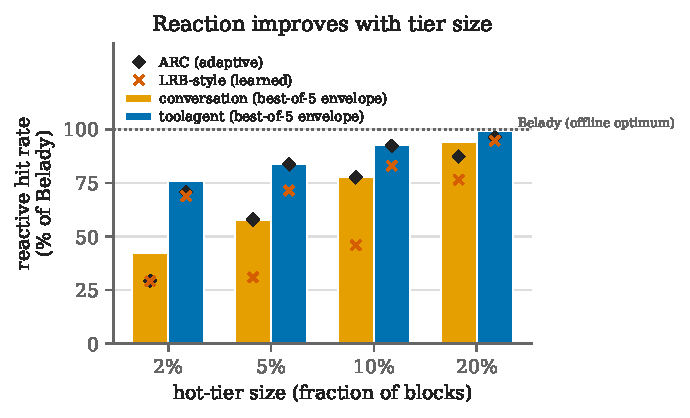
\includegraphics[width=\columnwidth]{fig_reactive.pdf}
  \caption{Reactive tiering as a fraction of Belady's hit rate, full Mooncake traces. Bars are a
  per-operating-point best-of-seven envelope, an oracle over policies rather than a policy. Diamonds are
  ARC, which meets the envelope at 5\% on both traces and at 10\% on conversation but falls short
  elsewhere; crosses are the
  LRB-style learned policy, which is below ARC everywhere.}
  \label{fig:reactive}
\end{figure}

\subsection{What the measurement required}
\label{sec:protocol}
Every positive result we obtained before the final protocol was an artifact, and each looked reasonable:
a flat captured fraction, a plausible interval, a learned policy landing below ARC. Two of the
twenty-seven defects in \Cref{tab:defects} were found by an adversarial review we ran with AI reviewer
agents (see the Acknowledgment), five by an audit and the rest by re-verification passes, all after the
paper had passed every check it defined for itself. The artifact's lab notebook records each one with
its fix.

\begin{table*}[t]
\centering\footnotesize
\begin{tabular}{@{}p{3.2cm}p{8.6cm}p{4.9cm}@{}}
\toprule
mechanism (count) & what happened & control now in the harness \\
\midrule
Reference-frame mismatch (6) & a split over access-event indices that fell past the trace's end; ties
broken by label (AUC 0.51 to 0.94); an oracle inheriting the heuristic's order; features built at one
split instant, costs billed at another & one split instant for features, labels and bill; frames compared
explicitly \\
Retracted claims (3) & retracted: a ``+66--88\% captured'' agentic headline that sampling showed was never
measurable; the \emph{decoupling} claim, an artifact of an unreachable denominator; an LRB column that
measured random eviction because its training buffer was truncated & randomized draws; the reachable
share beside any captured fraction; LRB fails on zero label variance \\
Free-parameter extrapolation (3) & curves read from one point: a cache size, a trace length, a
conversation count (+88\% reversing to $-48\%$) & every convenience parameter swept \\
Believing a report (1) & an edit script printed success after matching nothing & edits asserted to land \\
Stale derived or parallel surfaces (3) & artifacts older than the code that made them; figures fifteen
days older than their data; a notebook stating a falsified claim & content-hash provenance; figure and
PDF manifests; banners on records \\
Unchecked summaries (1) & a sentence misquoted a checked band's width & spans and maxima asserted;
withdrawn values must be absent \\
Unverified interventions (1) & a mutation whose target string was absent ``passed'' & interventions
asserted to apply; guards tested both ways \\
Emphasis without verification (1) & the headline share sat in no artifact and mixed two references
(97\% to 95\%, then 84--88\%) & every emphasised number asserted \\
Leaks and unstated conventions (8) & in the arrival experiment: post-split labels; a cut unlike the bill;
magnitudes from evaluation blocks' futures; zero beliefs for pre-split blocks; a mixed-scale ceiling; an
order control that also changed magnitude; unstated tie and action-space conventions (up to 56 points);
creations billed as reads (the gap inflated about three times) & a causal module with an AST taint test;
conventions swept; billable access defined in one place \\
\bottomrule
\end{tabular}
\caption{The twenty-seven measurement defects, by mechanism. Each produced a plausible number that matched
its artifact.}
\label{tab:defects}
\end{table*}

Two of them changed what this paper claims. A headroom taken at 1{,}500 requests moved by full length
from 86.4\% to 91.8\% on toolagent and from 82.9\% to 93.5\% on conversation, and a protocol evaluated
on short traces would have found far more reachable than the full traces show (\Cref{sec:reachable}).
And the conventions of \Cref{sec:arrival}, each fixed for convenience, moved one arm by up to 56 points.
Three controls would have caught most of the catalogue on the first day: compute the reachable share
beside any captured fraction; treat every convenience choice as a variable to sweep; and, before
reporting a null, compute the sample size that would have resolved it, because ``we could not tell'' and
``there is nothing there'' are different claims. The harness ships with these wired in, and with a
checker that re-derives every result in this paper from its artifact and fails on drift.

\subsection{Limitations}
\label{sec:limits}
No real vLLM+LMCache deployment was measured, so any cost-expressed quantity should be read as a range.
We tightened what that range means. Our first sensitivity analysis scaled every tier latency by a common
factor, which moves the absolute scale and leaves the \emph{ratios} between tiers untouched --- and the
ratios are what a placement policy responds to, so it never tested the parameter that mattered. We
therefore derive the table instead: KV bytes per block follow exactly from a model's attention shape
($2 \times \text{layers} \times \text{kv\_heads} \times \text{head\_dim} \times \text{dtype}$ per
token), and per-tier latency is that divided by a declared device-class bandwidth plus a fixed overhead.
Sweeping three attention shapes against five device classes puts headroom at \textbf{55--98\%}, which
contains the 92\% our hand-written table gives --- the headroom conclusion survives (we did not rerun the
unreachable share or the arrival arms under the derived tables), but two things about the
table do not. Its GPU:CPU latency ratio is 1:10 where every device class but the deliberately flat one gives 1:80 to 1:250, an order of
magnitude in the ratio the policy is most sensitive to; and \textbf{6 of the 15 configurations reorder
the hierarchy} so that latency order and capacity order disagree, which our fixed per-tier capacity table
cannot express at all. Calibrating against a live deployment remains the open gate; this is the honest
intermediate, not a substitute. The
\emph{timing} and \emph{representation} axes of \Cref{sec:formulation} are chosen by the simulator from
placeholder cost tables but carry no signal from the traces, which is why \Cref{sec:arrival} also reports
tier-only placement. A
representation pilot over three textual fidelities is in the artifact, but it depends on
a paid hosted model, and this paper reports only what the artifact regenerates without one. Both
sources are KV-block hash streams from transformer prefix caching, so they are independent in provenance
but not in mechanism. Alibaba's four traces (16-token blocks) and Mooncake's synthetic control broaden the
set, but we still cannot separate workload character from vendor, date, or block size. Sampling is not randomized, every placement result is
a single deterministic run, and no confidence interval is reported for them, though trace length, split
instant, cost weights, tie convention and action space are now swept rather than fixed. The arrival-time
arms form beliefs causally but are allocated capacity in one static assignment, which is neither a bound
nor an admission policy: replayed online they need nearly free migration to keep their gain (above).
The hazard estimate fixes one pseudo-split, its count bins and its age quartiles, and applies counts from
half the prefix to counts over the whole of it; rescaling for that moves the hazard arm by at most 0.6 points on the production traces. Of the learned and adaptive cache literature we evaluate
ARC~\cite{S7_megiddo2003arc}, LeCaR~\cite{S8_vietri2018lecar}, CACHEUS~\cite{S9_rodriguez2021cacheus} and
a reimplementation of LRB~\cite{S6_song2020lrb}; Hawkeye, Mockingjay and Baleen are positioned in
\Cref{sec:related} but not run, the first two because a KV block hash carries no analogue of the program
counter their predictors are indexed by. Our LRB is the
published mechanism rebuilt from the paper, not the authors' artifact (as are our LeCaR and CACHEUS, whose
CR-LFU expert we approximate by LFU), and the uniform block size of both sources removes one of LRB's
advantages over LRU, so the underperformance we report should be read as a statement about this workload
rather than about these designs.
